\documentclass[11pt,a4paper]{article}
\usepackage{od,amsmath}
\usepackage[utf8]{inputenc}
\usepackage[ngerman]{babel}

\newcommand{\xx}[2]{\parbox{#1\textwidth}{\vspace*{3pt}\centering
    #2\vspace*{3pt}}}
\newcommand{\br}[1]{\left(#1\right)}


\title{Gemeinsamkeiten und Unterschiede von TRIZ,\\ künstlicher
  Intelligenz und Kybernetik\\ als wissensbasierte Methoden\\ für die Lösung
  technischer Probleme}

\author{Dietrich Balzer, Friedrichsthal}
\date{10.\,01.\,2017}

\begin{document}
\maketitle

\begin{quote}
  Der Aufsatz wurde bei LIFIS-Online im Themenbereich \emph{Innovation und
    Systematisches Erfinden} am 10.01.2017 publizizert.  DOI:
  \url{http://dx.doi.org/10.14625/balzer_20170110}
\end{quote}

\section*{1.  Einleitung}

Eine vergleichende Analyse von TRIZ (Teoria reschenija isobretatelskich
zada\v{c} -- Lösung von Erfindungsaufgaben), Künstlicher Intelligenz (KI) und
Kybernetik ist bis heute nur in Ansätzen durchgeführt worden. So hat zum
Beispiel G.V. Sokolov vom „Institut für Systeme der Informatik“ der sibirischen
Abteilung der russischen Akademie der Wissenschaften in Novosibirsk unter der
Überschrift „Theorie der Entscheidungsfindung“ eine Darstellung verschiedener
systemtheoretischer Methoden einschließlich TRIZ vorgenommen ohne allerdings
eine vergleichende Analyse durchzuführen, vgl. [Sokolov 2015]. Zu erwähnen ist
in diesem Zusammenhang auch die Darstellung von V. Petrov, der über die
Technische Kybernetik zu TRIZ gelangt ist und der zu Fragen der
„Innovationstechnologie“ eine zusammenfassende Darstellung vorgelegt hat,
allerdings auch ohne die Zusammenhänge zwischen den verschiedenen
Innovationstechnologien zu untersuchen, vgl. [Petrov 2014].

Während die gemeinsame wissensbasierte Herangehensweise für TRIZ, Künstliche
Intelligenz und Kybernetik charakteristisch ist, bestehen andererseits
wesentliche Unterschiede, wie aus Tabelle 1 zu entnehmen ist.

\begin{figure}[ht]
\begin{center}\small
  \begin{tabular}{|l|l|l|l|}\hline
 & \xx{.25}{\bf Inhalt des Lösungsprozesses} & \xx{.22}{\bf Dynamik des
      Lösungsprozesses} & \xx{.25}{\bf Technische Umsetzung}\\\hline

\xx{.15}{\bf TRIZ} & \xx{.25}{Widersprüche als dialektisches Prinzip, ca. 40
  innovative Grundprinzipien (Zerlegung, Integration, Rükkopplung u.a.)} &
\xx{.22}{keine Echtzeitfähigkeit} & \xx{.25}{Rechnergestützte Off"|line-Lösung
  mit dem Ziel einer Erfindung (CAI)}\\\hline

\xx{.15}{\bf Künstliche Intelligenz} & \xx{.25}{Phänomenologische (Experten-
  und Fuzzysysteme) und biologische (neuronale Netze) Nachbildung des
  menschlichen Denkprozesses} & \xx{.22}{Echtzeitfähigkeit möglich} &
\xx{.25}{In Automatisierungs- und Steuerungssysteme integrierbar mit dem Ziel
  einer Systemoptimierung, enge Beziehung zur technischen Kybernetik}\\\hline

\xx{.15}{\bf Kybernetik} & \xx{.25}{Informationsgewinnung, -verarbeitung und
  -nutzung, online-Kopplung mit dem Steuerungsobjekt}&
\xx{.22}{Echtzeitfähigkeit unbedingt notwendig}& \xx{.25}{Prozessleitsysteme,
  Nutzung virtueller Automatisierungsnetze}\\\hline
  \end{tabular}\vskip1em\normalsize

  \textbf{Tabelle 1:} Vergleich von TRIZ, Künstlicher Intelligenz\\ und
    Kybernetik (Eigene Darstellung)
\end{center}
\end{figure}

Es liegt auf der Hand, dass ein Informations- und Erfahrungsaustausch zwischen
den Vertretern der drei Disziplinen für alle von Nutzen sein könnte. Der
vorliegende Beitrag soll ein praktischer Schritt in diese Richtung sein. Im
Weiteren werden folgende Probleme behandelt:
\begin{itemize}
\item Gegenstand der Kybernetik und der Künstlichen Intelligenz vom Standpunkt
  einer Kooperation mit TRIZ.
\item Zwei praktische Beispiele von wissensbasierten Systemen, deren Betrieb
  mit Hilfe von TRIZ verbessert werden konnte.
\item Methodik der mathematischen Modellierung zur Gewinnung von
  Tiefenwissen. 
\item Gegenseitiger Nutzen aus der Kooperation von TRIZ, künstlicher
  Intelligenz und Kybernetik.
\end{itemize}

Auf eine zusätzliche Darstellung der vom sowjetischen Wissenschaftler Genrich
Saulovitsch Altschuller entwickelten TRIZ-Theorie wird an dieser Stelle
verzichtet. Es wird in diesem Zusammenhang auf die große Anzahl von Vorträgen
auf der 21. Leibnizkonferenz des LIFIS am 24. und 25. November 2016 in
Lichtenwalde zu TRIZ und seiner Anwendung\footnote{Siehe
  \url{http://leibniz-institut.de/konferenzen}.}  hingewiesen. Diese Vorträge
werden bzw. wurden bereits in LIFIS online veröffentlicht. Zusätzlich sei
darauf hingewiesen, dass vor kurzem ein Artikel über den Lebensweg von
Altschuller als Forscher und Hochschullehrer anlässlich seines
90. Geburtstages veröffentlich wurde, vgl. [Gorelik 2016].

Die beiden oben genannten praktischen Beispiele beziehen sich auf
erfinderische Problemstellungen in der Prozessindustrie (Katalytische
drucklose Verölung mit Sauerstoff"|injektion, Nutzung von Restwärme zur
Stromerzeugung) durch eine Kooperation von TRIZ, Künstlicher Intelligenz und
Kybernetik mit dem Ziel einer Patentanmeldung. Dabei wird über die Erfahrungen
berichtet, die zwei Konsortien aus dem EuReffuS-Netzwerk\footnote{Siehe
  \url{http://www.eureffus.com}.} bei der Planung und teilweise bereits bei der
Realisierung automatisierter nachhaltiger Lösungen gesammelt hat.
  
\section*{2. Gegenstand der Kybernetik und der Künstlichen Intelligenz vom
  Standpunkt einer Kooperation mit TRIZ} 

Die Aufgaben der Kybernetik sind in Tabelle 2 zusammenfassend beschrieben. Auf
eine Darstellung der Prozessüberwachung als selbstständige
Prozesssteuerungsaufgabe wird an dieser Stelle verzichtet, da das eigentliche
Ziel der Kybernetik in der zielgerichteten Beeinflussung des
Steuerungsobjektes im Sinne der Prozesssicherung, -stabilisierung und
-optimierung besteht.

\begin{figure}[ht]
\begin{center}\small
  \begin{tabular}{|l|l|l|l|}\hline
 \xx{.25}{\bf Steuerungsfunktion} & \xx{.3}{\bf Verbale Erläuterung des
   Inhaltes} & \xx{.3}{\bf Typische technische Lösungen}\\\hline

 \xx{.25}{\bf Prozesssicherung} & \xx{.3}{Alarmierung, Notabschaltung bei
   Gefahrenzuständen, Verwirklichung von Abwehrstrategien, Verhinderung von
   Fehlbedienungen} & \xx{.3}{Sicherheits- und Schutzverriegelungssysteme,
   Abfahrsteuerungen auf Basis schaltungsprogrammierter Steuerungstechnik,
   intelligente vorbeugende Prozesssicherung}\\\hline

 \xx{.25}{\bf Prozessstabilisierung} & \xx{.3}{Automatische Kompensation von
   Störungsauswirkungen, dynamische Entkopplung von Teilsystemen} &
 \xx{.3}{Regelsysteme, intelligente Prozesskoordinierung}\\\hline

 \xx{.25}{\bf Prozessoptimierung} & \xx{.3}{Bestimmung und Einstellung
   optimaler Betriebsregime (Arbeitspunkte) \newline Bestimmung und
   Realisierung optimaler Übergangsvorgänge (Umstellen, Anfahren usw.)} &
 \xx{.3}{Einsatz von Optimierungsalgorithmen}\\\hline

  \end{tabular}\vskip1em\normalsize

  \textbf{Tabelle 2:} Steuerungsfunktionen als Aufgaben der Kybernetik (Eigene
  Darstellung)
\end{center}
\end{figure}
Die Methoden der Kybernetik basieren auf der Einheit von Steuerungssystem und
Steuerungsobjekt. Aus diesem Grund werden auch die Aufgaben des
Steuerungssystems durch eine vergleichende Analyse der Amplitude und der
Frequenz der auf das Steuerungsobjekt einwirkenden Störgrößen bestimmt (siehe
Abbildung 1). Darüber hinaus zeigt die Abbildung 1, dass mit sinkender Frequenz
der Störgrößen ein Einsatz von Systemen der künstlichen Intelligenz
(Expertensysteme) sinnvoll ist. Die gleiche Aussage trifft auch auf den Einsatz
von TRIZ-Methoden und auf den Einsatz des Menschen als Regler (Offener Kreis)
zu.
  
\begin{figure}[htp]
\begin{center}
  \includegraphics[width=.6\textwidth]{Bild_1.jpg}\vskip1em
  
  \textbf{Abbildung 1:} Ableitung von Steuerungsaufgaben (Eigene Darstellung)
\end{center}
\end{figure}
Bei der Darstellung der Methoden der Künstlichen Intelligenz gehen wir davon
aus, dass in erster Linie echtzeitfähige Expertensysteme für die
Prozesssteuerung zum Einsatz kommen, deren Grundstruktur seit 1992 Bestand hat
und auf Abbildung~2 gezeigt wird, vgl. [Balzer et al. 1992]. Der Entwickler
und der Benutzer des Expertensystems ist oft ein und dieselbe Person.

\begin{figure}[htp]
\begin{center}
  \includegraphics[width=.6\textwidth]{Bild_2.png}\vskip1em

\textbf{Abbildung 2:} Echtzeitfähige Expertensysteme zur Lösung\\ von
Steuerungsaufgaben, vgl. [Balzer et al. 1992].
\end{center}
\end{figure}
In Tabelle 3 werden die Funktionen der Komponenten des auf Abbildung 2
dargestellten Expertensystems erläutert.

\begin{figure}[htp]
\begin{center}\small
  \begin{tabular}{|l|l|l|}\hline
\xx{.25}{\bf Grundkomponente} & \xx{.25}{\bf Grundfunktion} & \xx{.4}{\bf
  Erläuterung} \\\hline

\xx{.25}{\bf Wissensbasis} & \xx{.25}{Wissensrepräsentation} & \xx{.4}{enthält
  das anwendungsspezifische Wissen} \\\hline

\xx{.25}{\bf Problemlösungs\-komponente} & \xx{.25}{Wissensmanipulation} &
\xx{.4}{beruht auf Theorien und Strategien zur Lösung von Aufgaben in
  bestimmten Problemklassen} \\\hline

\xx{.25}{\bf Akquisitions\-komponente} & \xx{.25}{Wissensakquisition} &
\xx{.4}{unterstützt den Experten bei der Entwicklung von Wissensbasen} \\\hline

\xx{.25}{\bf Erklärungs\-komponente} & \xx{.25}{Erklärung} & \xx{.4}{erklärt dem
  Entwickler bzw. Nutzer einen Lösungsweg} \\\hline

\xx{.25}{\bf Dialog\-komponente} & \xx{.25}{Dialog} & \xx{.4}{kommuniziert mit
  dem Entwickler bzw. Nutzer} \\\hline
  \end{tabular}\vskip1em\normalsize
  
\textbf{Tabelle 3:} Erläuterung der Funktionen des Expertensystems (Eigene
Darstellung)
\end{center}
\end{figure}

Die online erfassten Prozessdaten der zu steuernden und zu beobachtenden
technologischen Anlage werden als fallspezifisches Faktenwissen in die
Wissensbasis übertragen. Das anwendungsspezifische Expertenwissen besitzt
folgende Wissensformen:
\begin{itemize}
\item \emph{Assoziatives Oberflächenwissen} als logische Beziehungen zwischen
  Prozessmerkmalen und Schlussfolgerungen in Form von Regeln: Symptome --
  Situationen, Situationen -- Steuerungen, Steuerungen -- Wirkungen);
\item \emph{Qualitatives Tiefenwissen} als relationale Modelle der Struktur
  (Abstraktion, Aggregation, Kopplung, Sicht) und Funktion (Kausalketten,
  Normalverhalten, Fehlverhalten) von Steuerungsobjekt und  Steuerungssystem;
\item \emph{Quantitatives Tiefenwissen} als analytische Modelle des Systems
  (Mathematische Modelle für die Beschreibung von Übertragungsverhalten und
  Zustandsverhalten). 
\end{itemize}
Dieses Wissen spielt bei einer Kooperation mit TRIZ-Methoden eine wichtige
Rolle.  Wäh"|rend das Oberflächenwissen in der Regel aus Erfahrungen des
Betreibers der Anlage abgeleitet wird, stellt das Tiefenwissen das Ergebnis
einer mathematisch-naturwissenschaftlichen Analyse des Steuerungsobjektes dar.

Ein Beispiel für assoziatives Oberflächenwissen bezogen auf die Steuerung der
im Punkt 3 beschriebenen KDV-Anlage ist:
\begin{quote}
  \emph{Wenn} Temperatur in der Friktionsturbine höher als 250 Grad
  Celsius,\\ \emph{dann} Drehzahl herabsetzen \emph{und} Sauerstoffzufuhr
  reduzieren.
\end{quote}

\begin{figure}[htp]
\begin{center}
  \includegraphics[width=.6\textwidth]{Bild_3.jpg}\vskip1em

  \begin{quote}
    \textbf{Abbildung 3:} Beispiel für qualitatives Tiefenwissen (Eigene
    Darstellung).\\  $z_n$ -- Vektor der Störgrößen, $u_n$ -- Vektor der
    Steuergrößen, $y_n$ -- Vektor der Ausgangsgrößen
  \end{quote}
\end{center}
\end{figure}

Abbildung 3 zeigt als allgemeines Beispiel für qualitatives Tiefenwissen die
Struktur eines aus 3 Teilsystemen bestehenden Gesamtsystems.  Der Punkt 4
enthält Beispiele für quantitatives Tiefenwissen ebenfalls bezogen auf die im
Punkt 3 dargestellte KDV-Anlage.  Tabelle 4 beschreibt die Vor- und Nachteile
der verschiedenen Wissensformen.

\begin{figure}[htp]
\begin{center}\small
  \begin{tabular}{|l|l|l|}\hline
\xx{.22}{\bf Wissensform} & \xx{.3}{\bf Vorteile} & \xx{.3}{\bf Nachteile}
\\\hline

\xx{.22}{Assoziatives Oberflächenwissen} & \xx{.3}{Integration von Erfahrungen
  (Einfache Modellierbarkeit), mittlerer Rechenaufwand (gute
  Echtzeitfähigkeit), explizites Wissen (Regeln, gute Erklärbarkeit) } &
\xx{.3}{höhere Spezialisierung (eingeschränkte Wiederverwendbarkeit), Erfassung
  aller Fälle notwendig (Vollständigkeit nicht garantiert) } \\\hline

\xx{.22}{Qualitatives Tiefenwissen} & \xx{.3}{höhere Universalität (gute
  Wiederverwendbarkeit), Erfassung auch unvorgesehener Fälle (Vollständigkeit),
  explizites Wissen (gute Erklärbarkeit) } & \xx{.3}{hoher Rechenaufwand
  (eingeschränkte Echtzeitfähigkeit), Darstellung einfacher Zusammenhänge
  (eingeschränkte Modellierbarkeit von Zusammenhängen) } \\\hline

\xx{.22}{Quantitatives Tiefenwissen} & \xx{.3}{Darstellung komplizierter
  Zusammenhänge (gute Nachbildung durch mathematische Modelle, Ableitung von
  Regeln), verwendbar für Simulation, Projektierung und Steuerung (hohe
  Adäquatheit der Modelle) } & \xx{.3}{hoher Rechenaufwand (eingeschränkte
  Echtzeitfähigkeit), implizites Wissen (schwierige Erklärbarkeit).  } \\\hline
  \end{tabular}\vskip1em\normalsize
  
\textbf{Tabelle 4:} Vor- und Nachteile der verschiedenen Wissensformen (Eigene
Darstellung)
\end{center}
\end{figure}

Wichtig ist ein Vergleich der Strukturierung und Verarbeitung von Wissen bei
TRIZ, der Künstlichen Intelligenz und der Kybernetik für die Gestaltung der
Schnittstellen zwischen den Software-Paketen dieser drei Disziplinen
(siehe Tabelle 5).

\begin{figure}[htp]
\begin{center}\small
  \begin{tabular}{|l|l|l|}\hline
 & \xx{.22}{\bf Struktur des Wissens} & \xx{.3}{\bf
      Wissensmanipulation}\\\hline

\xx{.22}{TRIZ} & \xx{.3}{Widerspruchstabelle, innovative Vorgehensprinzipien
  (ca. 40)} & \xx{.3}{Logik, CAI}\\\hline

\xx{.22}{Künstliche Intelligenz und Kybernetik} & \xx{.3}{Oberflächenwissen
  (Regeln), Tiefenwissen (prozedural, mathematische Modelle)} & \xx{.3}{Logik,
  Expertensystemschalen}\\\hline 
  \end{tabular}\vskip1em\normalsize

  \begin{quote}
    \textbf{Tabelle 5:} Darstellung und Verarbeitung von Wissen bei TRIZ,
    Künstlicher Intelligenz und Kybernetik (Eigene Darstellung)
  \end{quote}
\end{center}
\end{figure}

An dieser Stelle soll der Begriff „Echtzeitfähigkeit“ erläutert werden. Im
Unterschied zu vielen Veröffentlichungen, in denen die Echtzeitfähigkeit als
Schnelligkeit interpretiert wird, verstehen wir unter Echtzeitfähigkeit die
Rechtzeitigkeit der Reaktion der Steuerungssysteme auf ein Ereignis
(Störungen).  Die Zeit-Dienste-Funktionen in der Abbildung 4 stellen die
Anforderungen an die Echtzeitfähigkeit in der Prozessindustrie symbolisch dar.
Die Antwortzeit auf ein Ereignis als zusätzliche Totzeit, hervorgerufen durch
die Informationsverarbeitung der Algorithmen der Kybernetik, der künstlichen
Intelligenz oder der TRIZ, darf bei der Prozesssicherung einen bestimmten Wert
(Deadline $t_d$) nicht überschreiten, um eine Havarie zu verhindern. Bei der
Prozessstabilisierung und bei der Prozessoptimierung hingegen wird der Gewinn,
der als rote Linie dargestellt ist, immer kleiner in Abhängigkeit von der
wachsenden Antwortzeit.

\begin{figure}[htp]
\begin{center}
  \includegraphics[width=.6\textwidth]{Bild_4.png}\vskip1em

  \begin{quote}
    \textbf{Abbildung 4:} Zu Fragen der Echtzeitfähigkeit bei der Anwendung von
    Methoden der Kybernetik, der künstlichen Intelligenz und der TRIZ (Eigene
    Darstellung)
  \end{quote}
\end{center}
\end{figure}
\section*{3. Katalytische drucklose Verölung mit
  Sauerstoff"|injektion} 

\subsection*{3.1 Bisherige Technologie} 
                                      
Das bisherige technologische Schema der katalytischen drucklosen Verölung ist
auf Abbildung 5 dargestellt.

\begin{figure}[htp]
\begin{center}
  \includegraphics[width=.75\textwidth]{Bild_5.png}\vskip1em
                    
  \begin{quote}
    \textbf{Abbildung 5:} Bisheriges Prinzipschema der Technologie zur
    katalytischen drucklosen Verölung (vgl. [Alphakat, Vesper, Aumos, TUD
      2015])
  \end{quote}
\end{center}
\end{figure}

Für dieses verfahrenstechnische System der katalytischen drucklosen Verölung
(KDV) besitzt die Firma Alphakat GmbH ein Hauptpatent DE 100\,49\,377 und
mehrere weitere Patente der letzten Jahre. Diese KDV-Anlage zur Erzeugung von
Diesel aus organischen Abfällen soll in ein virtuelles Kraftwerk (Mikrogrid)
integriert werden. Die vor Ort in einem BHKW aus Diesel erzeugte Energie (Strom
und Wärme) wird auch vor Ort genutzt. Teuere Energietrassen entfallen.
Gleichzeitig werden im Vergleich zu zentralen Energieerzeugungsanlagen die
Transportkosten für die Input-Stoffe drastisch reduziert.

Zentrale Elemente der KDV-Anlage sind eine Turbine (Turbogenerator) für die
Erzeugung von Diesel, ein Separator und eine Destillationskolonne zur Trennung
des Diesels von den übrigen Kohlenwasserstoffen (siehe Abbildung 6).


\begin{figure}[htp]
\begin{center}
  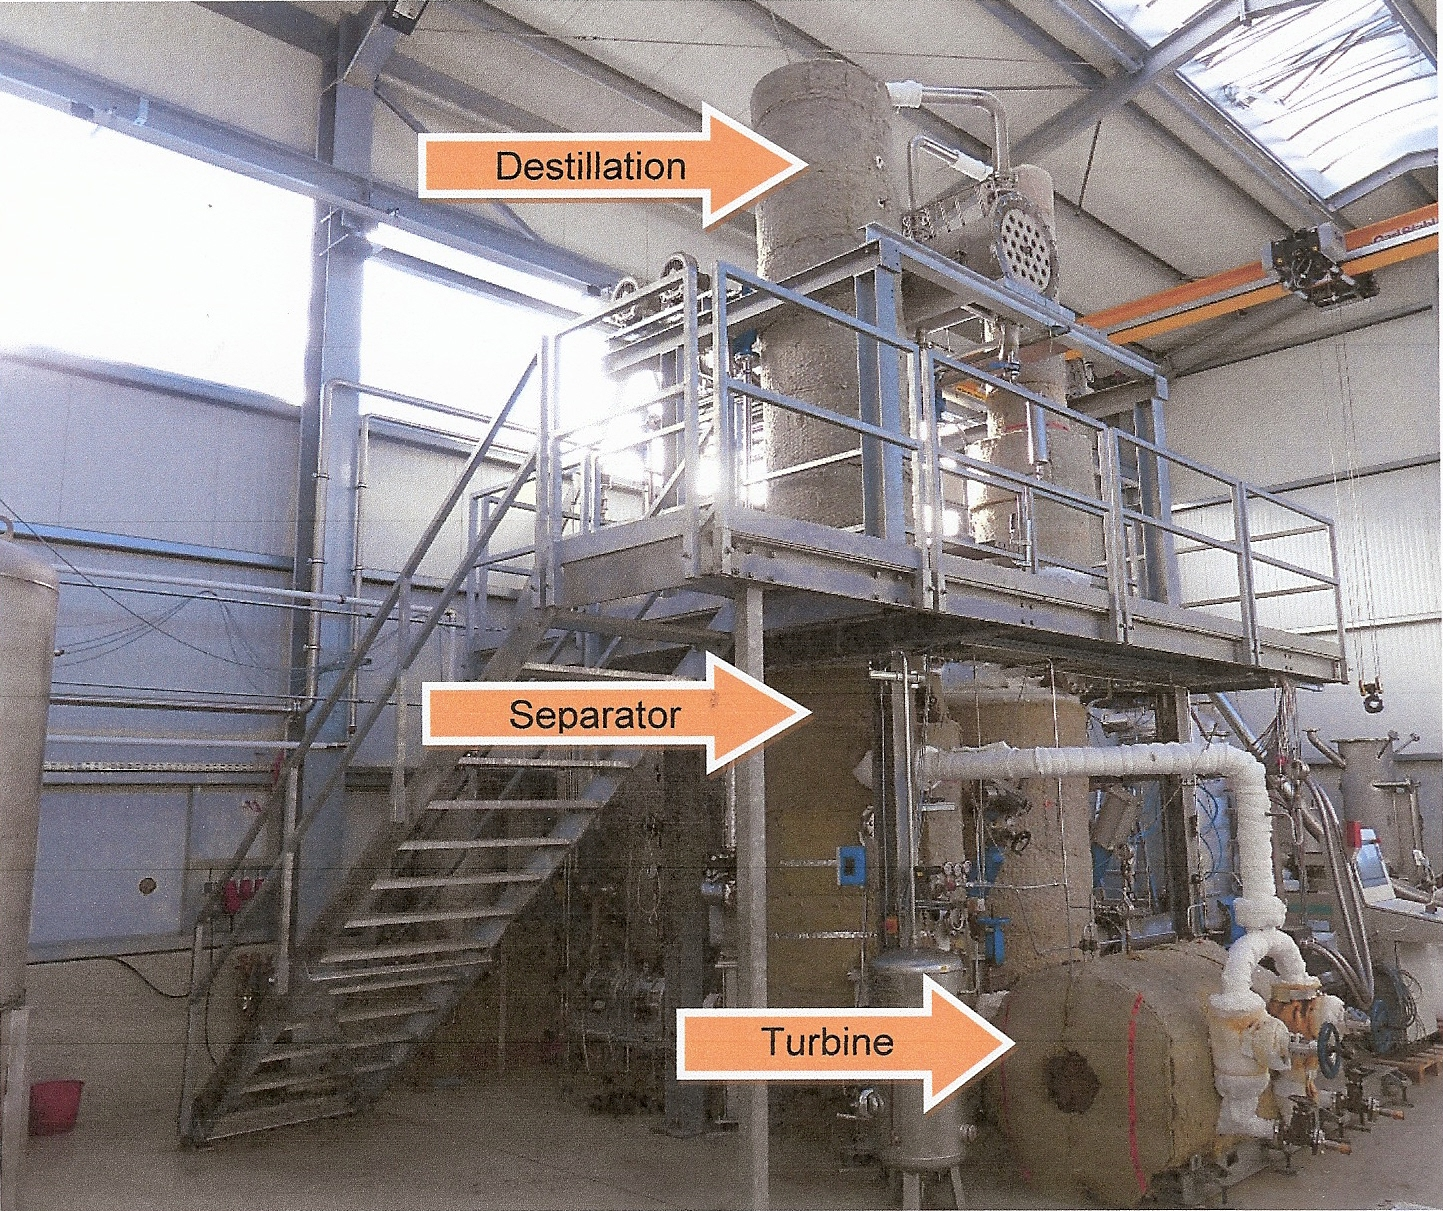
\includegraphics[width=.6\textwidth]{Bild_6.png}\vskip1em
             
  \textbf{Abbildung 6:} Außenansicht der KDV-Anlage\\ (vgl. [Alphakat, Vesper,
    Aumos, TUD 2015])
\end{center}
\end{figure}

In der Turbine laufen tribochemische katalytische Reaktionen der
Stoffumwandlung vor allem als Depolymerisation und Polymerisation ab. Die
chemische Summengleichung der Depolymerisation ohne Beachtung der
stöchiometrischen Koeffizienten lautet
\begin{center}
  Kunststoff ($C_{50}H_{96}$) + Zellulose ($C_6H_{11}O_5$) = Diesel
  ($C_{14}H_{28}$) + Kohlendioxyd ($CO_2$).
\end{center}
Die chemische Summengleichung der Polymerisation ebenfalls ohne Beachtung der
stöchiometrischen Koeffizienten lautet:
\begin{center}
  Zellulose ($C_6H_{11}O_5$) = Diesel ($C_{14}H_{28}$) + Kohlendioxyd ($CO_2$)
  + Wasserstoff ($H$).
\end{center}
Hauptmerkmale der bisherigen verfahrenstechnischen Anlage auf der Basis des
oben genannten Patentes sind:
\begin{itemize}
\item Katalytische Prozesse laufen bei niedrigen Temperaturen ab;
\item Keine Bildung von Dioxinen (Umweltschutz);
\item Inputstoffe sind sowohl biogene (Stroh, Holz u.a.) als auch
  hochkalorische (Kunststoffe u.a.) Abfall- und Reststoffe.
\end{itemize}

Beim Betreiben dieser Anlage traten folgende Probleme auf:
\begin{itemize}
\item Die Produktivität der Anlage ist zu gering.
\item Für die Erzeugung von Regelenergie in einem virtuellen Kraftwerk sind die
  möglichen Änderungsbereiche der Leistungsparameter zu gering.
\item Die Änderungsgeschwindigkeit der produzierten Dieselmenge pro Zeiteinheit
  ist auf Grund der großen Totzeiten und Zeitkonstanten für die Erzeugung von
  Regelenergie nicht ausreichend gering.
\end{itemize}

\subsection*{3.2 Dialektische Widersprüche und innovative Grundprinzipien bei
  der Entwicklung von Zusatzpatenten} 

Zur Lösung der im Punkt 3.1 beschrieben Probleme beim Betreiben der Anlage
wurden für die Rekonstruktion und für das Betreiben der Anlage TRIZ-Methoden in
Kombination mit Methoden der Künstlichen Intelligenz und der Kybernetik
eingesetzt. Im Laufe des Lösungsprozesses wurden folgende \emph{dialektische
Widersprüche} behandelt.

Der \emph{Widerspruch zwischen Sollwert und Istwert} beim Betreiben einer
technologischen Anlage ist ein charakteristischer dialektischer Widerspruch in
der Prozessindustrie. Das trifft natürlich auch auf die katalytische drucklose
Verölung zu. Der Sollwert ist eine zeitabhängige Funktion, die als Vorgabe für
einen zu messenden Istwert dient. In unserem Fall ist das z.B. der Durchsatz an
Diesel am Ausgang der Destillationskolonne in Abhängigkeit von der Zeit.

Der \emph{Widerspruch zwischen Zuverlässigkeit und Wartungsaufwand} besteht
darin, dass aus ökonomischen Gründen die Zuverlässigkeit der technologischen
Anlage, bestehend aus Steuerungsobjekt und Steuerungssystem, zu erhöhen und der
Wartungsaufwand für Hardware und Software zu reduzieren ist.

Der \emph{Widerspruch zwischen Funktionalität und Bedienkomfort} ist darauf
zurückzuführen, dass mit steigender Anzahl und Kompliziertheit der durch den
Operator zu verwaltenden Funktionen des Steuerungssystems, die ihrerseits
gleichzeitig miteinander verknüpft sind, die Übersichtlichkeit und Sicherheit
bei der Einschätzung von Situationen zunehmend verloren geht. Das führt dazu,
dass die Gefühlswelt des Operators durch Stress und Angst bestimmt wird, was
zwangsläufig zu einer Reduzierung der Zuverlässigkeit der
Operator-Prozess-Kommunikation führt.

Zur Lösung dieser Widersprüche wurden folgende innovative Grundprinzipien
eingesetzt:
\begin{itemize}
\item Dynamisierung des Gesamtsystems und seiner Teile
\item Einführung von Rückkopplungen
\item Zerlegung des Gesamtsystems in Teilsysteme
\item Universalität durch Nutzung von quantitativem Tiefenwissen (Mathematische
  Modelle) 
\item Veränderung der physikalischen und chemischen Eigenschaften
\item Anwendung starker Oxydationsmittel
\item Prinzip des „Vermittlers“
\end{itemize}
 Aus den oben beschriebenen dialektischen Widersprüchen wurde als erstes der
 Widerspruch bzw. die fehlende Übereinstimmung zwischen Sollwert und Istwert
 behandelt. Dabei spielten die innovativen Grundprinzipe \emph{Veränderung der
   physikalischen und chemischen Eigenschaften} und \emph{Anwendung starker
   Oxydationsmittel} eine entscheidende Rolle. Unter Nutzung der Kenntnisse und
 Erfahrungen aus anderen katalytischen Prozessen mit Gleichgewichtsreaktionen
 wurden die Eigenschaften der Inputstoffe und damit der Zwischen- und
 Endprodukte dahingehend geändert, dass durch die Zuführung von Sauerstoff
 erstens eine Beschleunigung der katalytischen Reaktionen erreicht wurde und
 dass zweitens durch den Sauerstoff als starkes Oxydationsmittel hervorgerufene
 Oxydationsprozesse eine zusätzliche Wärmezuführung erfolgte. Das hatte den
 Vorteil, dass die Produktivität der Anlage um ca. 30\,\% erhöht wurde. Um den
 Ort und die Menge der Zufuhr von Sauerstoff genau zu bestimmen wurde das
 innovative Grundprinzip \emph{Universalität durch Nutzung von quantitativem
   Tiefenwissen (Mathematische Modelle)} in Form von mathematischen Modellen
 angewendet. Dadurch war es möglich, die wesentlichen Eigenschaften einer
 Friktionsturbine mit Sauerstoff"|injektion vorherzusagen und gleichzeitig die
 konstruktiven Parameter der Friktionsturbine zu bestimmen (s. Abbildung 7).
 
\begin{figure}[htp]
\begin{center}
  \includegraphics[width=.6\textwidth]{Bild_7.png}\vskip1em

   \textbf{Abbildung 7:} Neue Turbine mit Sauerstoff"|injektion\\ (vgl.
          [Alphakat, Vesper, Aumos, TUD 2015])
 \end{center}
\end{figure}

Das war die Grundlage für ein Zusatzpatent.  Als weitere innovative
Grundprinzipien wurden die \emph{Einführung von Rückkopplungen} und die
\emph{Dynamisierung des Gesamtsystems und seiner Teile} verwendet. Dabei wurde
nach den Regeln der Kybernetik die Differenz von Soll- und Istwert als
Eingangssignal für einen Informationsverarbeitungsalgorithmus verwendet. Das
Ausgangssignal dieses Algorithmus dient als Steuergröße. Diese beiden
Prinzipien führten zur Schaffung eines Systems der zentralen Steuerung
dezentraler Anlagen zur katalytischen drucklosen Verölung mit
Sauerstoff"|injektion (s. Abbildung 8), was ein weiteres Zusatzpatent
darstellt.


\begin{figure}[htp]
\begin{center}
  \includegraphics[width=.9\textwidth]{Bild_8.png}\vskip1em
  
  \begin{quote}
    \textbf{Abbildung 8:} Zentrale Steuerung dezentraler Anlagen zur
    katalytischen drucklosen Verölung mit Sauerstoff"|injektion (Eigene
    Darstellung)
  \end{quote}
\end{center}
\end{figure}

Die notwendigen Elemente bei der Lösung der Automatisierungsaufgaben führen
dazu, dass die Struktur des Automatisierungs- und Steuerungssystems der
KDV-Anlage eine zweistufige Hierarchie besitzen (siehe Abbildung 8). Dazu
wurde im Rahmen eines EU-Forschungsprojektes die Konzeption für „Virtual
Automation Networks (VAN)“ entwickelt, in dem sowohl öffentliche und private
als auch industrielle Kommunikationstechnologien zu einem einzigen
skalierbaren System mit einer im Idealfall garantierten Dienstgüte (Quality of
Service – QoS) integriert werden können (rot gekennzeichnet: VAN enabled;
vgl. [VAN 2009]).

Die praktischen Vorteile der zentralen Steuerung und Wartung dezentraler
technologischer Anlagen mit Hilfe eines Operatorzentrums sind:
\begin{itemize}
\item Das Know-how eines Operators oder Wartungsingenieurs ist für viele
  Anlagen ohne Zeitverzögerung für die Lösung von Prozessführungsaufgaben
  einsetzbar.
\item Ein modellgestütztes Prozessführungssystem ist für viele Anlagen
  einsetzbar.
\item Die Kosten für die zentrale Leittechnik werden durch die Anzahl der
  dezentralen Anlagen geteilt.
\item Integration eines Trainingssimulators und eines CAI-Systems in die
  zentrale Leittechnik (e-Learning) ist möglich, wobei ein mathematisches
  Modell die Basis für die Anlagensimulation bildet.
\item Der geschätzte ökonomische Nutzen bei der Steuerung von KDVi-Anlagen
  beträgt unter Beachtung der Erfahrungen in der Verfahrenstechnik
  (z.B. Abfallwirtschaft, Nutzung erneuerbarer Energien) eine etwa
  dreißigprozentige Gewinnerhöhung.
\end{itemize}

Die Aufgaben der TRIZ-Software (CAI, computer aided innovation) als Bestandteil
des Operatorzentrums bestehen einmal in der Unterstützung des Operators bei der
Neubestimmung der Prozessführungsaufgaben:
\begin{itemize}
\item Vergleichende Analyse der Eigenschaften der Störgrößen (Frequenz und
  Amplitude) und der Eigenschaften des Steuerungsobjektes (Dynamische
  Charakteristika der Stör- und Steuerkanäle) mit dem Ziel der Bestimmung der
  Prozessführungsaufgaben (Prozessoptimierung, -stabilisierung und
  -sicherung). 
 \item Echtzeitfähige Lösung der Prozessführungsaufgaben
   (Prozessoptimierung, -stabili"|sierung und -sicherung) durch die Lösung von
   Widersprüchen zwischen Sollwerten und Istwerten bei Temperaturen,
   Durchsätzen und Drücken.
\end{itemize}
Zum anderen geht es um die Unterstützung des Projektanten bei der
Neuentwicklung des Turbogenerators mit Sauerstoff"|injektion:
\begin{itemize}
\item Konstruktion des neuen Turbogenerators und Formulierung eines Patentes
\item Erstellung der Fertigungsunterlagen
\end{itemize}

Bei der Lösung des Widerspruchs zwischen Zuverlässigkeit und Wartungsaufwand
wurde das innovative Grundprinzip \emph{Zerlegung des Gesamtsystems in
  Teilsysteme} angewendet. Nur durch diese Zerlegung in Teilsysteme kann eine
Berechnung und Optimierung der Zuverlässigkeit des Gesamtsystems durchgeführt
werden. Darüber hinaus macht eine solche Zerlegung eine sinnvolle Wartung und
eine Ermittlung des Wartungsaufwandes erst möglich. Durch die jetzt mögliche
quantitative Bewertung der Zuverlässigkeit und des Wartungsaufwandes kann eine
Systemoptimierung erfolgen.

Die Behandlung des Widerspruches zwischen Funktionalität und Bedienkomfort
erfordert, wie bei der Bearbeitung des Widerspruches zwischen Soll- und
Istwert, den Einsatz des innovativen Grundprinzips \emph{Universalität durch
  Nutzung von quantitativem Tiefenwissen (Mathematische Modelle)}, denn nur
adäquate mathematische Modelle können die Funktionalität nachbilden. In diesem
Sinne könnte man auch die mathematische Modellierung als Anwendung des
innovativen Grundprinzips \emph{Prinzip des Vermittlers} bezeichnen, denn das
mathematische Modell „vermittelt“ zwischen Steuerungsobjekt und Operator. In
der Kybernetik spricht man dabei von modellbasierter Steuerung.

Diese Nachbildung ist auch notwendig um den Bedienkomfort abschätzen und
optimieren zu können. Außerdem wird das Grundprinzip \emph{Zerlegung des
Gesamtsystems in Teilsysteme} zur Verbesserung der Übersichtlichkeit und damit
zur Verbesserung des Bedienkomforts angewendet. Hier soll auf die Arbeit von
A.M. Dvorjakin und R.R. Romanenko bezüglich der Generierung von Ideen bei der
Lösung von Erfindungsaufgaben in der Programmierung zur Lösung des Widerspruchs
zwischen Funktionalität und Bedienkomfort hingewiesen werden (vgl. [Dworjankin,
Romanenko 2012]).

Das eigentliche Ziel bei der Lösung des Widerspruchs zwischen Funktionalität
und Bedienkomfort ist die Optimierung der Mensch-Prozess-Schnittstelle im Sinne
der Maximierung der Zuverlässigkeit dieser Schnittstelle. Dabei spielen beim
Einsatz der TRIZ-Software folgende Gesichtspunkte eine Rolle:
\begin{itemize}
\item Verwendung kognitiver Bilder (optische und akustische Darstellungen) für
  die Beschreibung von Situationen in der Anlage (z.B. Weltkugel, Darstellung
  der Natur, Gesichtsausdrücke für Freude, Wut, Ekel, Furcht, Verachtung,
  Traurigkeit, Überraschung u.a.);
\item Unterstützung des menschlichen Problemlösungsprozesses
  (Wissensakquisition, -prä"|sentation, -manipulation, -konsultation);
\item Anpassung des Operator Interface an die kognitiven und sensormotorischen
  Fähigkeiten des Menschen durch Lösung von Widersprüchen (CAI); 
\item Schaffung einer Multimedia-Schnittstelle ohne praktische technische
  Beschränkungen (Hier: bimediale Schnittstelle: Sprache und Visualisierung); 
\item Realisierung einer Doppelstrategie: den Menschen auf Maschinen trainieren
  und die Maschine auf den Menschen einstellen.
\end{itemize}
Diese Gesichtspunkte beschreiben auch das Zusammenwirken von kognitiver
Psychologie und TRIZ bei der Lösung von Aufgaben der Kybernetik.

\section*{4. Methodik der mathematischen Modellierung
  der Friktionsturbine} 

Das theoretische mathematische Modell, das die in der Friktionsturbine mit
Sauerstoff"|injektion ablaufenden chemisch-katalytischen und physikalischen
Prozesse beschreibt und universell nachbildet, basiert auf
Bilanzgleichungen. Die mathematische Modellierung ist damit eine Methode, mit
der ein innovatives Grundprinzip von TRIZ, nämlich die \emph{Universalität}, in
praktische Lösungen umgesetzt werden kann.  Die Abbildungen 9 und 10 zeigen die
bei der mathematischen Modellierung verwendeten Beziehungen.

\begin{figure}[htp]
\begin{quote}
  \fbox{\xx{.25}{Die zeitliche Änderung eines Stoffes $i$ im Volumen}} =
  \fbox{\xx{.25}{der durch Strömung zugeführten Stoffmenge $i$}} +
  \fbox{\xx{.25}{der durch Diffussion zugeführten Stoffmenge
      $i$}}\\[1.5em] \hspace*{.3\textwidth} +
  \fbox{\xx{.5}{der durch eine Quelle zugeführten Stoffmenge (für den Fall
      eines chemischen Reaktionssystems der im Verlauf von $m$ Reaktionen
      entstehenden Stoffmenge $i$).}}
\end{quote}
\begin{center}
  \textbf{Abbildung 9:} Materialbilanz (Eigene Darstellung)
\end{center}\vskip1em
\begin{quote}
  \fbox{\xx{.26}{Zeitlicher Zuwachs an Energie im Volumen $V$}} =
  \fbox{\xx{.25}{dem Volumen durch Strömung zugeführte Energie}} +
  \fbox{\xx{.25}{dem Volumen durch Leitung zugeführte
      Energie}}\\[1.5em] \hspace*{.28\textwidth} + \fbox{\xx{.25}{dem Volumen
      durch Diffusion zugeführte Energie}} + \fbox{\xx{.25}{dem Volumen durch
      chemische Reaktion zugeführte Energie.}}
\end{quote}
\begin{center}
  \textbf{Abbildung 10:} Energiebilanz (Eigene Darstellung)
\end{center}
\end{figure}

In Abhängigkeit von der Verweilzeitverteilung als universelle Charakteristik
der Hydrodynamik existieren in der Friktionsturbine drei Teilsysteme. Im
Bereich der Turbinenschaufeln haben wir ein System mit idealer Durchmischung.
In den Bereichen der Zuführung und der Abführung des Reaktionsgemisches haben
wir ein System mit eindimensionaler Diffusion in Bewegungsrichtung. Das
bedeutet, dass wir zwei Typenmodelle verwenden, die wir im Weiteren erläutert
werden:
\newpage

\begin{itemize}
\item Eindimensionales Diffusionsmodell für die Bereiche der Zuführung und
  Abführung des Reaktionsgemisches.
\item Ideales Mischungsmodell für den Bereich der Turbinenschaufeln.
\end{itemize}

Aus den Modellen der Zuführung des Reaktionsgemisches, des Raumes der
Turbinenschaufeln und der Abführung des Reaktionsgemisches wird ein
Gesamtmodell erstellt, indem diese drei Modelle in Reihe geschaltet werden.

\subsubsection*{Eindimensionales Diffusionsmodell}

Materialbilanzen:
\begin{gather*}
  \frac{\partial x_i}{\partial t} +w\,\frac{\partial x_i}{\partial l}
  +D_L\,\frac{\partial^2 x_i}{\partial l^2} =
  f_i(x_1,x_2,\ldots,x_i,\ldots,x_n,T),\ i=1,2,\ldots,n \tag{1}
\end{gather*}
mit
\begin{align*}
  & x_i(t,l)\ \text{-- Konzentration der Komponente $i$,}\\
  & T(t,l)\ \text{-- Temperatur,}\\
  & f_i(x_1,x_2,\ldots,x_i,\ldots,x_n,T)\ \text{-- Reaktionsgeschwindigkeit auf
    der Basis der }\\
  & \qquad\text{Formalkinetik bei Bildung bzw. Verbrauch der Komponente
    $X_i$,}\\ 
  & w\ \text{-- lineare Geschwindigkeit der Komponente in der
    Friktionsturbine,}\\
  & D_L\ \text{-- Längsvermischungskoeffizient in der Friktionsturbine,}\\
  & t\ \text{-- Zeit,}\\
  & l\ \text{-- laufende Länge des Reaktionsraumes der Friktionsturbine.}
\end{align*}
Der Koeffizient $D_L$ wird aus der geschätzten oder experimentell ermittelten
Verweilzeitverteilung $\phi(\tau)$ unter Verwendung folgender aus der
Hydrodynamik bekannten Gleichung bestimmt:
\begin{gather*}
  \phi(\tau)=\frac{w}{\sqrt{4\,\pi\,D_L\,\tau}}\,
  \exp\left(\frac{w^2\,\left(\tau-\frac{L}{w}\right)^2}{4\,D_L\,\tau}\right)
\end{gather*}
mit 
\begin{align*}
  & L\ \text{-- die Länge des Raums der Zuführung bzw. der Abführung des
    Reaktionsgemisches}\\ 
  & \tau\ \text{-- Verweilzeit}
\end{align*}

Energiebilanz:

\begin{gather*}
  \frac{\partial T}{\partial t} +w\,\frac{\partial T}{\partial l}
  +D_L\,\frac{\partial^2 T}{\partial l^2} =
  h_i\,f_i(x_1,x_2,\ldots,x_i,\ldots,x_n,T),\ i=1,2,\ldots,n \tag{2}
\end{gather*}
mit
\begin{align*}
  & T(t)\ \text{-- Temperatur,}\\
  & h_i\ \text{-- von der Wärmetönung der chemischen Reaktion und von der
    spezifischen}\\
  &\qquad \text{Wärmekapazität des aufzuheizenden Mediums abhängiger
    Koeffizient.} 
\end{align*}
      
\subsubsection*{Ideales Mischungsmodell}

Materialbilanzen:
\begin{gather*}
  \frac{{d}\,x_i}{{d}\,t} =\frac{V_i}{V_0}(x_i-x_{ie})
  +f_i(x_1,x_2,\ldots,x_i,\ldots,x_n,T),\ i=1,2,\ldots,n \tag{3}
\end{gather*}
mit
\begin{align*}
  & x_i(t)\ \text{-- Konzentration der Komponente $i$,}\\
  & T(t)\ \text{-- Temperatur,}\\
  & x_{ie}\ \text{-- Konzentration der Komponente $i$ am Eingang in die
    Friktionsturbine,}\\
  & V_i\ \text{-- Menge der zugeführten Komponente $i$ pro Zeiteinheit,}\\
  & V_0\ \text{-- Inneres Volumen der Friktionsturbine.}
\end{align*}

Wärmebilanz:
 \begin{gather*}
  \frac{{d}\,T}{{d}\,t} =\frac{\sum_i V_i}{V_0}\,c\,(T-T_{e}) +\sum_i
  g_i\,f_i(x_1,x_2,\ldots,x_i,\ldots,x_n,T) \tag{4}
\end{gather*}
mit
\begin{align*}
  & T_e\ \text{-- durch eine Mischungsgleichung zu bestimmende mittlere}\\
  & \qquad\text{Eingangstemperatur aller Komponenten,}\\
  & c\ \text{-- Spezifische Wärme des Mediums im Reaktionsraum,}\\
  & g_i\ \text{-- von der Wärmetönung der chemischen Reaktion und von der
    spezifischen}\\
  & \qquad\text{Wärmekapazität des aufzuheizenden Mediums abhängiger
    Koeffizient.}
\end{align*}

Sowohl für das eindimensionale Diffusionsmodell als auch für das ideale
Mischungsmodell wurden für folgende Komponenten Bilanzgleichungen unter
Verwendung der Beziehungen (1) bis (4) aufgestellt:
\begin{quote}
  Kunststoff ($C_{50}H_{96}$), Zellulose ($C_6H_{11}O_5$), Diesel
  ($C_{14}H_{28}$), Kohlendioxid ($CO_2$), Wasserstoff ($H_2$), Sauerstoff
  ($O_2$).
\end{quote}
Für beide Modelle müssen noch die Anfangs- und Randbedingungen formuliert
werden, was aber grundsätzlich keine Schwierigkeiten bereitet. Außerdem sind
noch die Wärmeverluste in der Zu- und Abführung in Gleichung (2) zu bestimmen.
Darüber hinaus muss noch die durch Reibung der Turbinenschaufeln mit dem
Reaktionsgemisch zugeführte  Wärme in Gleichung (4) berechnet werden. Die Menge
an zugeführtem Sauerstoff als Funktion der Zeit  geht in die  Randbedingungen
ein.

Eine Simulation bzw. Nachbildung des dynamischen und statischen Verhaltens der
Friktionsturbine mit dem Ziel der Prozessoptimierung, -stabilisierung und
-sicherung sowie der Prognose erfolgt durch gleichzeitige Lösung der oben
dargestellten Differentialgleichungssysteme (1) bis (4).

\section*{5. Restwärmenutzung zur Stromerzeugung}

\subsection*{5.1 Konzept der Umwandlung von Restwärme in elektrische Energie}

Es geht in diesem Fall um einen neuen Ansatz zur Erhöhung der
Energieeffizienz. Die bei vielen industriellen Prozessen anfallende „Abwärme“
bzw. „Restwärme“ in Form von thermischer Energie auf aus energietechnischer
Sicht niedrigem Temperaturniveau (weniger als $300\,^\circ\mathrm{C}$,
„Niedertemperaturwärme“) soll für die Elektroenergiegewinnung nutzbar gemacht
werden. Um Technologien für die Nutzbarmachung immer niedriger temperierter
„Abwärme“ letztlich als Produkt erfolgreich platzieren zu können, benötigt man
einen innovativen Ansatz und eine kostengünstige Lösung mit verbesserten
technischen Parametern.

Ausgehend von dieser Einschätzung wurde die Patentanmeldung der Fa. PA Future
beim DPMA mit dem Aktenzeichen 10\,2013\,104\,868.4 „Anordnung und Verfahren zur
Umwandlung von Niedertemperaturwärme in mechanische Energie“ als
aussichtsreicher Ansatz für die Entwicklung einer neuen Variante zur Gewinnung
von Elektroenergie aus Niedertemperaturwärme identifiziert.

Laut Patentbeschreibung besteht die Aufgabe der Erfindung in einer effizienten
Umwandlung von Niedertemperaturwärme in mechanische bzw. elektrische
Energie. Insbesondere sollen die Kondensationswärme in Kraftwerken, Abwärme und
solar erzeugte Wärme als Energiequelle zu Bereitstellung mechanischer Energie
genutzt werden können.

Das Verfahren zur Umwandlung von Niedertemperaturwärme in mechanische Energie
arbeitet mit einem gasförmigen Arbeitsmittel – vorrangig verdichteter
Außenluft. Dazu wird von einer Wärmequelle Wärme mittels Wärmeübertrager auf
das verdichtete Gas, insbesondere Luft, übertragen. Dabei dehnt sich das Gas
aus, was zu einer Volumenvergrößerung und/oder Druckerhöhung des Gases
führt. Nachfolgend wird das erwärmte Gas in einer Kraftmaschine entspannt und
dabei mechanische Arbeit zur Erzeugung elektrischer Energie verrichtet.

Die Vorteile dieses Konzeptes gegenüber den bekannten Lösungen (ORC-Prozess,
Stirling-Maschinen u.a.) sind:
\begin{itemize}
\item Keine Beschränkungen bezüglich des Temperaturniveaus des Heizmediums
  bzw. der Restwärmequelle. 
\item Arbeitsmedium Luft ist überall kostenlos verfügbar.
\item Offener thermodynamischer Kreislauf ohne Kühlung des Arbeitsmediums,
  dadurch hoher Wirkungsgrad. 
\end{itemize}
In einem Heizkraftwerk soll dieses Konzept prototypisch umgesetzt werden
(s. Abbildung 11).  

\begin{figure}[htp]
\begin{center}
  \includegraphics[width=.8\textwidth]{Bild_11.png}\vskip1em

  \textbf{Abbildung 11:} Nutzung von Niedertemperaturwärme in einem\\
    Heizkraftwerk (HKW) zur Stromerzeugung (vgl. [ILK, Kunz, GAD 2016])
\end{center}
\end{figure}
Erhebliche Mengen an Niedertemperatur-Abwärme fallen in konventionellen
Heizkraftwerken an. Dort wird durch die Verbrennung von Rohbraunkohle
Elektroenergie und Wärmeenergie erzeugt. Mit der Wärme kann ein großer Teil
einer Stadt mit Heizwärme und Warmwasser versorgt werden.

In einem abgeschlossenen System der Energieumwandlung wird zunächst im
konventionellen Dampfturbinenprozess Dampf erzeugt, um eine Turbine für die
Elektroenergie-Erzeugung anzutreiben. Nachdem der Dampf die Turbine verlassen
hat, ist dieser entspannt und muss kondensiert werden. Dazu wird der Dampf
durch einen Wärmetauscher geleitet, der das Wasser der Heiztrasse für die
Wärmeversorgung aufheizt. Dem Dampf wird die Energie entzogen, er kondensiert
und kann wieder erhitzt werden, um ihn erneut als Dampf der Turbine
zuzuführen. Damit gestaltet sich die Erzeugung von Elektroenergie abhängig von
der Möglichkeit, den entspannten Dampf kondensieren zu lassen, mit anderen
Worten: eine energieeffiziente Produktion von Elektroenergie ist nur möglich,
wenn ausreichend Heizwärme abgenommen wird.

Um diesem Zustand abzuhelfen und die Elektroenergieerzeugung kontinuierlich und
unabhängig von den Jahreszeiten gestalten zu können, soll eine Anlage
entwickelt werden, die als Regelungs- bzw. Ausgleichselement in diesem Prozess
fungiert und dabei idealerweise noch weitere Elektroenergie erzeugen kann. Mit
der zu entwickelnden Anlage könnten sowohl die Dampferzeugung als auch die
Erzeugung von Elektroenergie erheblich verstetigt werden. Wird im Wärmetauscher
eine zu geringe Temperaturdifferenz zwischen abgegebenem und rückgeführtem
Dampf erreicht, wird ein Teil des Dampfes umgeleitet und durch das zu
schaffende Regelungselement dem Dampf Wärme entzogen. Die Abbildung 11 ist eine
konkrete Untersetzung dieser Lösungsprinzips unter Nutzung von
Rotationskolbenmaschinen (vgl. [ILK, Kunz, GAD 2016]).  

\subsection*{5.2 Machbarkeitsanalyse}

Der Motor und der Verdichter sind mit einer starren Welle verbunden. Es ist die
Frage zu beantworten, wie hoch der zu erwartende Wirkungsgrad bzw. die
Machbarkeit der Anlage zur Restwärmenutzung ist. Zu diesem Zweck wurde der
zugrunde liegende Kreislaufprozess thermodynamisch analysiert. Den
entsprechenden Prozessverlauf (Übergänge zwischen vier thermodynamischen
Zuständen) zeigt die Abbildung 12.

\begin{figure}[htp]
\begin{center}
  \includegraphics[width=.6\textwidth]{Bild_12.png}\vskip1em

 \textbf{Abbildung 12:} Thermodynamische Analyse\\ des Prozessverlaufs
 (vgl. [ILK, Kunz, GAD 2016])
\end{center}
\end{figure}

Um die im Prozess der Restwärmenutzung gewonnene Arbeit zu ermitteln,
betrachten wir die Übergänge zwischen den in Fehler: Referenz nicht gefunden
dargestellten Zuständen. Für die thermischen und energetischen Abschätzungen
wurden folgende Prozessberechnungen durchgeführt, die im Einzelnen aus
Platzgründen aber nicht dargestellt werden sollen:
\begin{quote}
  \emph{Isentrope Kompression} Zustand (1) $\to$ Zustand (2)
\end{quote}
Die Verdichtungsendtemperatur $T_2$ nach der isentropen Kompression berechnet
sich unter Nutzung der bekannten thermodynamischen Beziehungen aus der
Eintrittstemperatur $T_1$.
\begin{quote}
  \emph{Isobare Erwärmung} (2) $\to$ (3) 
\end{quote}
Die isobare Erwärmung der komprimierten Luft erfolgt in einem Wärmetauscher,
der einen Teil der Abwärme $q_{zu}$ an die komprimierte Luft überträgt. Dabei
werden Wärmebilanzgleichungen verwendet, die nach den auf der Abbildung 10
dargestellten Prinzipien erstellt wurden.
\begin{quote}
  \emph{Isentrope Expansion} (3) $\to$ (4)
\end{quote}
Die Endtemperatur $T_4$ nach der isentropen Expansion berechnet sich analog wie
bei der isentropen Kompression aus der Anfangstemperatur der Expansion $T_2$.
Aus der Differenz der Anfangs- und der Endtemperatur, der isochoren
spezifischen Wärmekapazität und dem Expander-Wirkungsgrad berechnet sich die
spezifische Abtriebsarbeit des Expanders $q_{ab}$.

Es treten folgende Probleme beim Betreiben der Lösung auf.

Bei 
\begin{gather*}
  q_{zu} \ge q_{ab}(W_{Nutz})+\text{Reibungsverluste} \tag{5}
\end{gather*}
erhöht sich die Drehgeschwindigkeit der Welle kontinuierlich (Fehlende
Stabilität), was zu einer Zerstörung des Systems führen kann.  Bei
\begin{gather*}
  q_{zu} \le q_{ab}(W_{Nutz})+\text{Reibungsverluste} \tag{6}
\end{gather*}
ist die Betriebsfähigkeit des Systems nicht gegeben.

Auf Grund dieser Probleme konnte das System der Restwärmenutzung zur
Stromerzeugung noch nicht realisiert werden. Es muss ein Steuerungssystem
entwickelt werden, mit dessen Hilfe die Bedingung   
\begin{gather*}
  q_{zu} = q_{ab}(W_{Nutz})+\text{Reibungsverluste} \tag{7}
\end{gather*}
erfüllt wird. 

\subsection*{5.3 Dialektische Widersprüche und Anwendung innovativer\\
  Grundprinzipien bei der Entwicklung eines Zusatzpatentes} 

Ohne das oben erwähnte Steuerungssystem kann die neue Lösung nicht betrieben
und nicht auf dem Markt angeboten werden, da die Stabilität des Gesamtsystems
und die geforderten Parameter nicht eingehalten werden können. Das ist vor
allem auf folgendes zurückzuführen:
\begin{itemize}
\item Die Zielfunktionen und die Nebenbedingungen sind nicht stationär sondern
  stark zeitabhängig. Eine Nachführung muss zeitoptimal und mit hoher
  Genauigkeit erfolgen. 
\item	Die Prozessgrößen „Durch den Verdichter transportierte Luftmenge pro
  Zeiteinheit“ und „Drehzahl der Welle“ besitzen eine positive Rückkopplung,
  was zu Instabilitäten führen kann. 
\item	Die beiden Wärmetauscher (Neue Lösung und HKW) sind technologisch in
  Reihe geschaltet. Das führt zu bedeutenden Totzeiten und Zeitkonstanten der
  Übertragungskanäle „Eingang in den neuen Wärmetauscher – Ausgang aus dem
  HKW-Wärmetauscher“. Um der Steuerung vorausschauenden Charakter zu verleihen,
  wird als Regelgröße nicht, wie allgemein üblich, die Temperatur am Ausgang
  des Wärmetauschers, sondern das Temperaturfeld über die Länge des
  Wärmetauschers benutzt. Nach dem gleichen Prinzip wird der Sollwert für diese
  Regelgröße berechnet.
\end{itemize}
Zur Lösung der oben beschriebenen Probleme beim Betreiben der Anlage wurden wie
auch bei der Rekonstruktion der KDV-Anlage für die Entwicklung des
Steuerungssystems als ein Zusatzpatent TRIZ-Methoden in Kombination mit
Methoden der Künstlichen Intelligenz und der Kybernetik eingesetzt.

Der Lösungsprozess wird durch  folgende \emph{dialektische Widersprüche}
charakterisiert.

Die Behandlung des \emph{Widerspruches zwischen Sollwert und Istwert}
entspricht im Prinzip der Vorgehensweise bei der KDV-Anlage.  Der Sollwert ist
in diesem Fall die Drehzahl der Welle als eine zeitabhängige Funktion, die als
Vorgabe für einen zu messenden Istwert dient.  Die Lösung dieses Widerspruchs
erfolgte mit Hilfe der innovativen Grundprinzipien \emph{Dynamisierung} und
\emph{Rückkopplung}. Damit wurde die erste Komponente des Steuerungssystems
geschaffen, die eine Kompensation der positiven inneren Rückkopplung des
Systems „Verdichter- Wärmetauscher-Motor-Generator“ durch ein wissensbasiertes
Prozessstabilisierungssystem unter Einhaltung der Bedingung (7) zum Ziel
hatte. Diese Kompensation erfolgte durch eine äußere negative informationelle
Rückkopplung.

Der \emph{Widerspruch zwischen Optimalität und Stabilität} wird in der
Prozessindustrie oft dadurch charakterisiert, dass das Optimum in der Nähe der
Stabilitätsgrenze liegt. Es kommt deshalb darauf an, beim Betrieben der Anlage
erstens die Steuergrößen mit hoher Genauigkeit zu bestimmen und zweitens das
Prozessoptimierungssystem mit einem Prozessstabilisierungssystem zu koppeln.

Die Entwicklung des Prozessoptimierungssysteme und seiner Kopplung mit dem
Prozessstabilisierungssystem erfolgte durch Anwendung der innovativen
Grundprinzipien \emph{Universalität durch Anwendung von quantitativem
  Tiefenwissen (Mathematische Modelle)} und \emph{Zerlegung}. Die
\emph{Zerlegung} war die Voraussetzung für die Modellierung der einzelnen
Elemente des Gesamtsystems.  Das Grundprinzip \emph{Anwendung der
  Wärmeausdehnung} ist die generelle Grundlage für das Konzept der Nutzung der
Restwärme zur Stromerzeugung. Die Ergebnisse bei der Lösung der Widersprüche
unter Anwendung der genannten innovativen Grundprinzipien kann wie folgt
zusammengefasst werden. Das System der Prozessführung bzw. Steuerung der Anlage
zur Restwärmenutzung wird nach verschiedenen Zielfunktionen in Abhängigkeit von
den sich dynamisch ändernden energetischen und wirtschaftlichen Anforderungen
an das Heizkraftwerk betrieben:
\begin{itemize}
\item Erzeugte Elektroenergiemenge pro Zeiteinheit;
\item zugeführte Dampfmenge pro Zeiteinheit;
\item kombinierte Zielfunktion (gewichtete Zielfunktionen): erzeugte
  Elektroenergiemenge pro Zeiteinheit und zugeführte Dampfmenge pro
  Zeiteinheit.
\end{itemize}
Dabei sind folgende technologische Größen bzw. Parameter automatisiert zu
erfassen, zu verarbeiten und zu optimieren:
\begin{itemize}
\item	Steuergrößen: 
\begin{itemize}
\item Durchsatz der Luftmenge pro Zeiteinheit am Eingang in den Wärmetauscher;
\item zugeführte Dampfmenge pro Zeiteinheit (kann auch Zielfunktion sein).
\end{itemize}
\item Regelgrößen: Temperaturfeld des Wärmetauschers (neues Prinzip: Regelung
  nach dem Temperaturfeld); Drehgeschwindigkeit der Welle.
\item Störgrößen:
\begin{itemize}
\item Variation der Sollwerte für die zu erzeugende Fernwärmemenge pro
  Zeiteinheit;
\item Variationen der Außenlufttemperatur;
\item Variationen der Zielfunktion;
\item Variationen der Nebenbedingungen.
\end{itemize}
\item Nebenbedingungen bzw. einzuhaltende Vorgaben:
  \begin{itemize}
  \item Erzeugte Fernwärmemenge pro Zeiteinheit unter Beachtung der kritischen
    Unterbrechungszeiten;
  \item vollständige Kondensierung des Dampfes am Ausgang aus dem Wärmetauscher
    des HKW;
  \item Begrenzung der Änderungsgeschwindigkeiten der zugeführten Dampfmenge
    nach der Zeit und der produzierten Elektroenergiemenge nach der Zeit.
  \end{itemize}
\end{itemize}
Aus der Beschreibung der Prozessführungsaufgabe geht hervor, dass zwei
intelligente Schnittstellen zu entwickeln sind:
\begin{itemize}
\item Schnittstelle zwischen Restwärmeproduzent (Heizkraftwerk) und der neuen
  Lösung mit dem Ziel der Bestimmung und Einstellung der zugeführten
  Wärmemenge pro Zeiteinheit;
\item Schnittstelle zwischen dem Generator der neuen Lösung und dem
  Elektroenergiesystem, das die erzeugte Elektroenergie aufnimmt.
\end{itemize}
Diese Prozessführungsaufgabe wird mit einem Steuerungssystem mit drei
Hierarchieebenen gelöst (siehe Tabelle 6). Die Struktur dieses Steuerungssystem
ist ähnlich der Struktur des VAN-basierte Systems auf Abbildung 8.

\begin{figure}[htp]
\begin{center}\small
  \begin{tabular}{|l|l|l|}\hline
    \xx{.23}{\bf Ebene} & \xx{.38}{\bf
      Informations\-verar\-bei\-tungs\-algorithmus} & \xx{.27}{\bf
      Bemerkungen}\\\hline

   \xx{.23}{\bf 1. Stabilisierung der Steuer\-größen} &
    \xx{.38}{Eindimensionale Festwertregelkreise mit linearen Reglern} &
    \xx{.27}{Einsatz von Standardkomponenten möglich}\\\hline

   \xx{.23}{\bf 2. Bestimmung der Sollwerte für die Regelgrößen} &
    \xx{.38}{Neuartige Steuerung des Wärmetauschers nach dem Temperaturfeld,
      mehrdimensionale nichtlineare Regelungssysteme, Beachtung der
      Nebenbedingungen bei der Optimierung der Sollwerte} & \xx{.27}{Keine
      Standardsysteme vorhanden, mathematische Modellierung der Dynamik des
      Wärmetauschers notwendig}\\\hline
    
   \xx{.23}{\bf 3. Auswahl der Zielfunktion und der Neben- bedingungen} &
    \xx{.38}{Nutzung von Elementen der künstlichen Intelligenz, Modellierung
      des Gesamtsystems Heizkraftwerks als neues System} & \xx{.27}{Keine
      Standardlösungen vorhanden}\\\hline
  \end{tabular}\vskip1cm\normalsize
  
  \begin{quote}
    \textbf{Tabelle 6:} Aufgaben des Steuerungssystems bei der Nutzung der
    Restwärme zur Stromerzeugung (Eigene Darstellung)
  \end{quote}
\end{center}
\end{figure}

\section*{6. Gegenseitiger Nutzen aus der Kooperation von TRIZ,
  künstlicher Intelligenz und Kybernetik}

An dieser Stelle soll ausgehend von Erfahrungen der in den Punkten 3, 4 und 5
beschrieben Beispielen der Nutzen der Kooperation der drei
Wissenschaftsdisziplinen zusammengefasst werden.

Die \emph{künstliche Intelligenz} und die \emph{Kybernetik} können für
\emph{TRIZ} folgendes leisten:
\begin{itemize}
\item Unterstützung der innovativen Grundprinzipien durch regelbasierte
  Systeme. 
\item Akquisition von Oberflächenwissen und Tiefenwissen zur Beschreibung
bzw. Auflösung von Widersprüchen.
\item Einsatz von Expertensystemschalen für die Entwicklung und den Betrieb von
  TRIZ-Systemen (CAI).
\end{itemize}
Dabei spielt die Erstellung der Wissensbasis die entscheidende Rolle. Dazu
werden Methoden des Wissensingenieurwesens verwendet. Das Wissensingenieurwesen
basiert auf einem Vier-Phasenkonzept:
\begin{itemize}
\item Definitionsphase
\item Akquisitionsphase
\item Operationalisierungsphase
\item Wartungsphase
\end{itemize}
Innerhalb der Definitionsphase wird eine Anforderungsspezifikation erarbeitet.
Mit anderen Worten: Es ist die Steuerungsaufgabe zu bestimmen:
Prozessstabilisierung, Prozessoptimierung oder Prozesssicherung.

In der Akquisitionsphase erfolgen eine Analyse der Störgrößen, der kausalen
Zusammenhänge innerhalb des Steuerungsobjektes und die Erstellung formaler
Modelle. In dieser Phase werden vor allem Methoden der Kybernetik eingesetzt.
Dabei geht es um eine „technologienahe Strukturierung“ des Wissens.

Während der Operationalisierungsphase wird das Wissen systemnah strukturiert.
Außerdem wird die Betriebsfähigkeit des Steuerungssystems als wissensbasiertes
System hergestellt.

In der Wartungsphase wird neu gewonnenes Wissen (z.B. in Form von neuen Regeln)
in die Wissensbasis eingefügt.

\emph{TRIZ} kann für die \emph{Kybernetik} folgendes leisten:
\begin{itemize}
\item Lösung von dialektischen Widersprüchen (z.B. zwischen Optimalität und
  Stabilität, zwischen Sollwert und Istwert);
\item Anwendung innovativer Grundprinzipien (z. B. Integration, Rückkopplung,
  Zerlegung, Dynamisierung)
\end{itemize}
Diese Leistungen führen zu einer wesentlichen Vereinfachung der Projektierung
und des Betreibens von technischen Systemen. Abbildung 13 zeigt das
diesbezügliche Zusammenwirken von TRIZ, Künstlicher Intelligenz und Kybernetik.

\begin{figure}[htp]
\begin{center}
  \includegraphics[width=.9\textwidth]{Bild_13.png}\vskip1em

  \begin{quote}
    \textbf{Abbildung 13:} Zusammenwirken von TRIZ, Künstlicher Intelligenz und
    Kybernetik bei der Planung und beim Betrieb von technischen Systeme (Eigene
    Darstellung).
  \end{quote}
\end{center}
\end{figure}
TRIZ und Künstliche Intelligenz bestimmen das Lösungsgebiet und schränken damit
den Lösungsraum ein, während die Kybernetik den Lösungspunkt definiert.
\newpage

\section*{7. Literatur}

\begin{itemize}
\item  Alphakat, Vesper, Aumos, TUD (2015): Automatisierte Anlage zur
  katalytischen drucklosen Verölung (Unveröffentlichte Projektbeschreibung).
\item  Balzer, D. et al. (1992): Wissensbasierte Systeme in der
  Automatisierungstechnik. Carl Hanser Verlag München Wien.
\item  Dvorjankin, A.M., Romanenko, R.R. (2012): Generatsia idej pri
  reschenii isobretatelskich sada\v{c} v programmirovanii (Generierung von
  Ideen bei der Lösung von Erfindungsaufgaben in der Programmierung).  Isvestia
  Volgogradskovo gosudarstvennovo techni\v{c}eskovo universiteta, 13.4.
\item  Gorelik, V. (2016): On dal \v{c}elove\v{c}estvy nitj Ariadny (Er gab
  der Menschheit den Faden der Ariadne).  Jevrejskaja panorama Nov. 2016.
\item  ILK, Kunz, GAD (2016): „Restwärmenutzung unter Verwendung einer
  Rotationskolbenmaschine“ (Unveröffentlichte Projektbeschreibung).
\item  Petrov, V. (2014); Technologija inovatsij
  (Innovationstechnologie). \\
  \url{http://temm.ru/file.php/id/f4508/name/Innovation\%20Technology-max.pdf}
\item  Sokolov, G.V. (2015): Sistemy poiska reschenij (Systeme der
  Entscheidungsfindung). \url{http://triz.iis.nsk.su/sokolov/dss-preface}.
\item  VAN (2009): EU-R\&D-Project „Virtual Automation Networks
  (VAN)”, Deliverable D09.2-1.
\end{itemize}
\end{document}
